\documentclass[tikz,border=12pt]{standalone}
\usepackage{amsmath,amssymb}
\usepackage{tikz}
\usetikzlibrary{arrows.meta,positioning,fit,calc,backgrounds}
\tikzset{
  box/.style={
    draw,
    very thick,
    rectangle,
    align=center,
    inner sep=8pt,
    minimum height=1.25cm,
    minimum width=3.1cm,
    font=\small,
  },
  wide/.style={box, minimum width=3.6cm},
  arr/.style={-{Stealth[length=2.6mm, width=2mm]}, thick},
  barr/.style={
    {Stealth[length=2.4mm, width=1.8mm]}-{Stealth[length=2.4mm, width=1.8mm]},
    thick,
  },
  lbl/.style={font=\scriptsize, inner sep=2pt, fill=white},
  group/.style={draw, dashed, inner sep=12pt},
}

\begin{document}
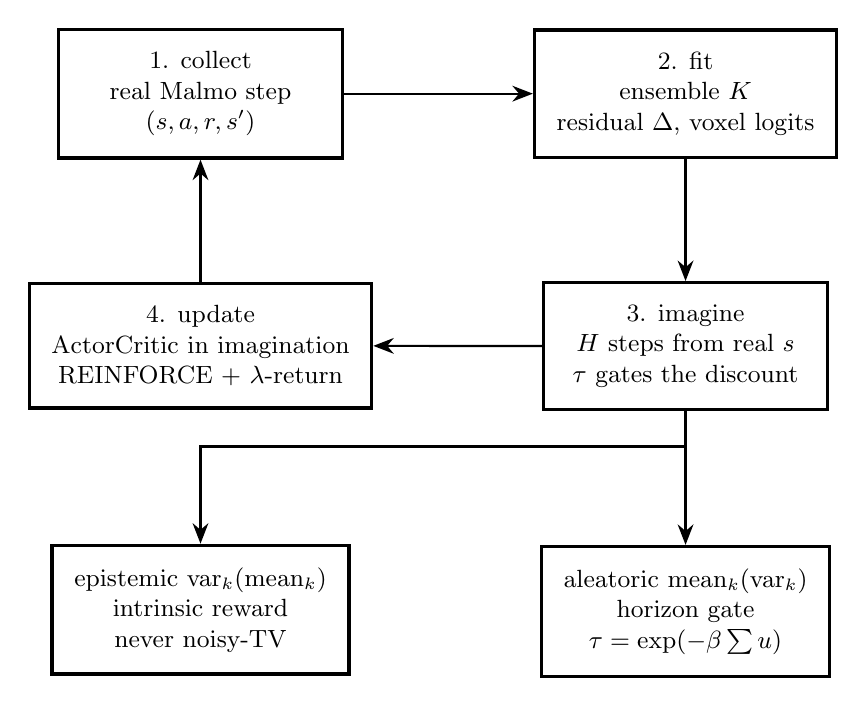
\begin{tikzpicture}[node distance=1.55cm and 2.4cm]
  \node[wide] (col) {1. collect\\real Malmo step\\$(s,a,r,s')$};
  \node[wide, right=of col] (fit) {2. fit\\ensemble $K$\\residual $\Delta$, voxel logits};
  \node[wide, below=of fit] (img) {3. imagine\\$H$ steps from real $s$\\$\tau$ gates the discount};
  \node[wide, below=of col] (upd) {4. update\\ActorCritic in imagination\\REINFORCE + $\lambda$-return};

  \draw[arr] (col) -- (fit);
  \draw[arr] (fit) -- (img);
  \draw[arr] (img) -- (upd);
  \draw[arr] (upd) -- (col);

  \node[wide, below=1.7cm of upd] (epi) {epistemic $\mathrm{var}_k(\mathrm{mean}_k)$\\intrinsic reward\\never noisy-TV};
  \node[wide, below=1.7cm of img] (ale) {aleatoric $\mathrm{mean}_k(\mathrm{var}_k)$\\horizon gate\\$\tau=\exp(-\beta\sum u)$};

  \draw[arr] (img.south) -- ++(0,-0.45) -| (ale.north);
  \draw[arr] (img.south) -- ++(0,-0.45) -| (epi.north);
\end{tikzpicture}
\end{document}
